\documentclass{article}

\usepackage{amsmath}
\usepackage{amsfonts}
\usepackage{amssymb}
\usepackage{multicol}

\usepackage{mathenv}
\usepackage{multirow}

\usepackage{vmargin}
\setmarginsrb{2.5cm}{2.5cm}{2.5cm}{2.5cm}{0cm}{0cm}{0cm}{0cm}

\usepackage[utf8]{inputenc}

\usepackage[french]{babel}
\selectlanguage{french}

\usepackage{color}
\usepackage{hyperref}
\hypersetup{pdfborder={0 0 0}, colorlinks=true, urlcolor=blue, linkcolor = darkred}
\usepackage{graphicx}
\graphicspath{{fab/}, {ant/}} 
\usepackage{listings}
\definecolor{colKeys}{rgb}{0.75,0,0}
\definecolor{colIdentifier}{rgb}{0,0,0}
\definecolor{colComments}{rgb}{0.75,0.75,0}
\definecolor{colString}{rgb}{0,0,0.7}

\usepackage{verbatim}
\usepackage{moreverb}

\lstset{
basicstyle=\ttfamily\small, %
identifierstyle=\color{colIdentifier}, %
keywordstyle=\color{colKeys}, %
stringstyle=\color{colString}, %
commentstyle=\color{colComments}, %
showspaces=false,
}
\lstset{language=java}

% Commandes personnelles %

\definecolor{darkred}{rgb}{0.85,0,0}
\definecolor{darkblue}{rgb}{0,0,0.7}
\definecolor{darkgreen}{rgb}{0,0.6,0}
\definecolor{darko}{rgb}{0.93,0.43,0}
\definecolor{maintitle}{rgb}{0.66,0,0.22}
\definecolor{title}{rgb}{0,0.5,0.5}
\newcommand{\maintitlecolor}[1]{\textcolor{maintitle}{#1}}
\newcommand{\titre}[1]{\textcolor{title}{#1}}
\newcommand{\tsect}[1]{\titre{\section{#1}}}
\newcommand{\tssect}[1]{\titre{\subsection{#1}}}
\newcommand{\tsssect}[1]{\titre{\subsubsection{#1}}}
\newcommand{\vect}[1]{\overrightarrow{#1}}
\newcommand{\dred}[1]{\textcolor{darkred}{\textbf{#1}}}
\newcommand{\dgre}[1]{\textcolor{darkgreen}{\textbf{#1}}}
\newcommand{\dblu}[1]{\textcolor{darkblue}{\textbf{#1}}}
\newcommand{\dora}[1]{\textcolor{darko}{\textbf{#1}}}
\newcommand{\gre}[1]{\textcolor{darkgreen}{#1}}
\newcommand{\blu}[1]{\textcolor{darkblue}{#1}}
\newcommand{\ora}[1]{\textcolor{darko}{#1}}
\newcommand{\rouge}[1]{\textcolor{darkred}{#1}}
\newcommand{\ceil}[1]{\left\lceil #1 \right\rceil}
\newcommand{\cdil}[1]{\left\lfloor #1 \right\rfloor}
\newcommand{\term}[1]{\textit{\textcolor{maintitle}{#1}}}
\newcommand{\image}[1]{\includegraphics{#1}}
\newcommand{\imageR}[2]{\includegraphics[width=#2px]{#1}}
\newcommand{\imageRT}[2]{\includegraphics[height=#2px]{#1}}
\newcommand{\img}[1]{\begin{center}\includegraphics[width=400px]{#1}\end{center}}
\newcommand{\imag}[1]{\begin{center}\includegraphics{#1}\end{center}}
\newcommand{\imgR}[2]{\begin{center}\includegraphics[width=#2px]{#1}\end{center}}
\newcommand{\imgRT}[2]{\begin{center}\includegraphics[height=#2px]{#1}\end{center}}
\newcommand{\point}[2]{\item \ora{\underline{#1}} : \textit{#2}}
\newcommand{\bfp}[2]{\item \textbf{#1} : \textit{#2}}
\newcommand{\sumparam}[3]{\sideset{}{_{#1}^{#2}}\sum{#3}}
\newcommand{\sumin}[3]{\sideset{}{_{i=#1}^{#2}}\sum{#3}}
\newcommand{\sumkn}[3]{\sideset{}{_{k=#1}^{#2}}\sum{#3}}
\newcommand{\intin}[3]{\sideset{}{_{#1}^{#2}}\int{#3}}
\newcommand{\stitre}[1]{\noindent\textbf{\underline{#1}} \\}
\newcommand{\R}{\mathbb{R}}
\newcommand{\Z}{\mathbb{Z}}
\newcommand{\N}{\mathbb{N}}
\newcommand{\ualpha}{\vect{u_\alpha}}
\newcommand{\valpha}{\vect{v_\alpha}}
\newcommand{\palpha}{\vect{\Psi_\alpha}}
\newcommand{\npcomp}{\term{$\mathcal{NP}$-complet}}
\newcommand{\npcompl}{\term{$\mathcal{NP}$-complet} }
\DeclareMathAlphabet{\mathpzc}{OT1}{pzc}{m}{it}

\begin{document}\begin{sffamily}

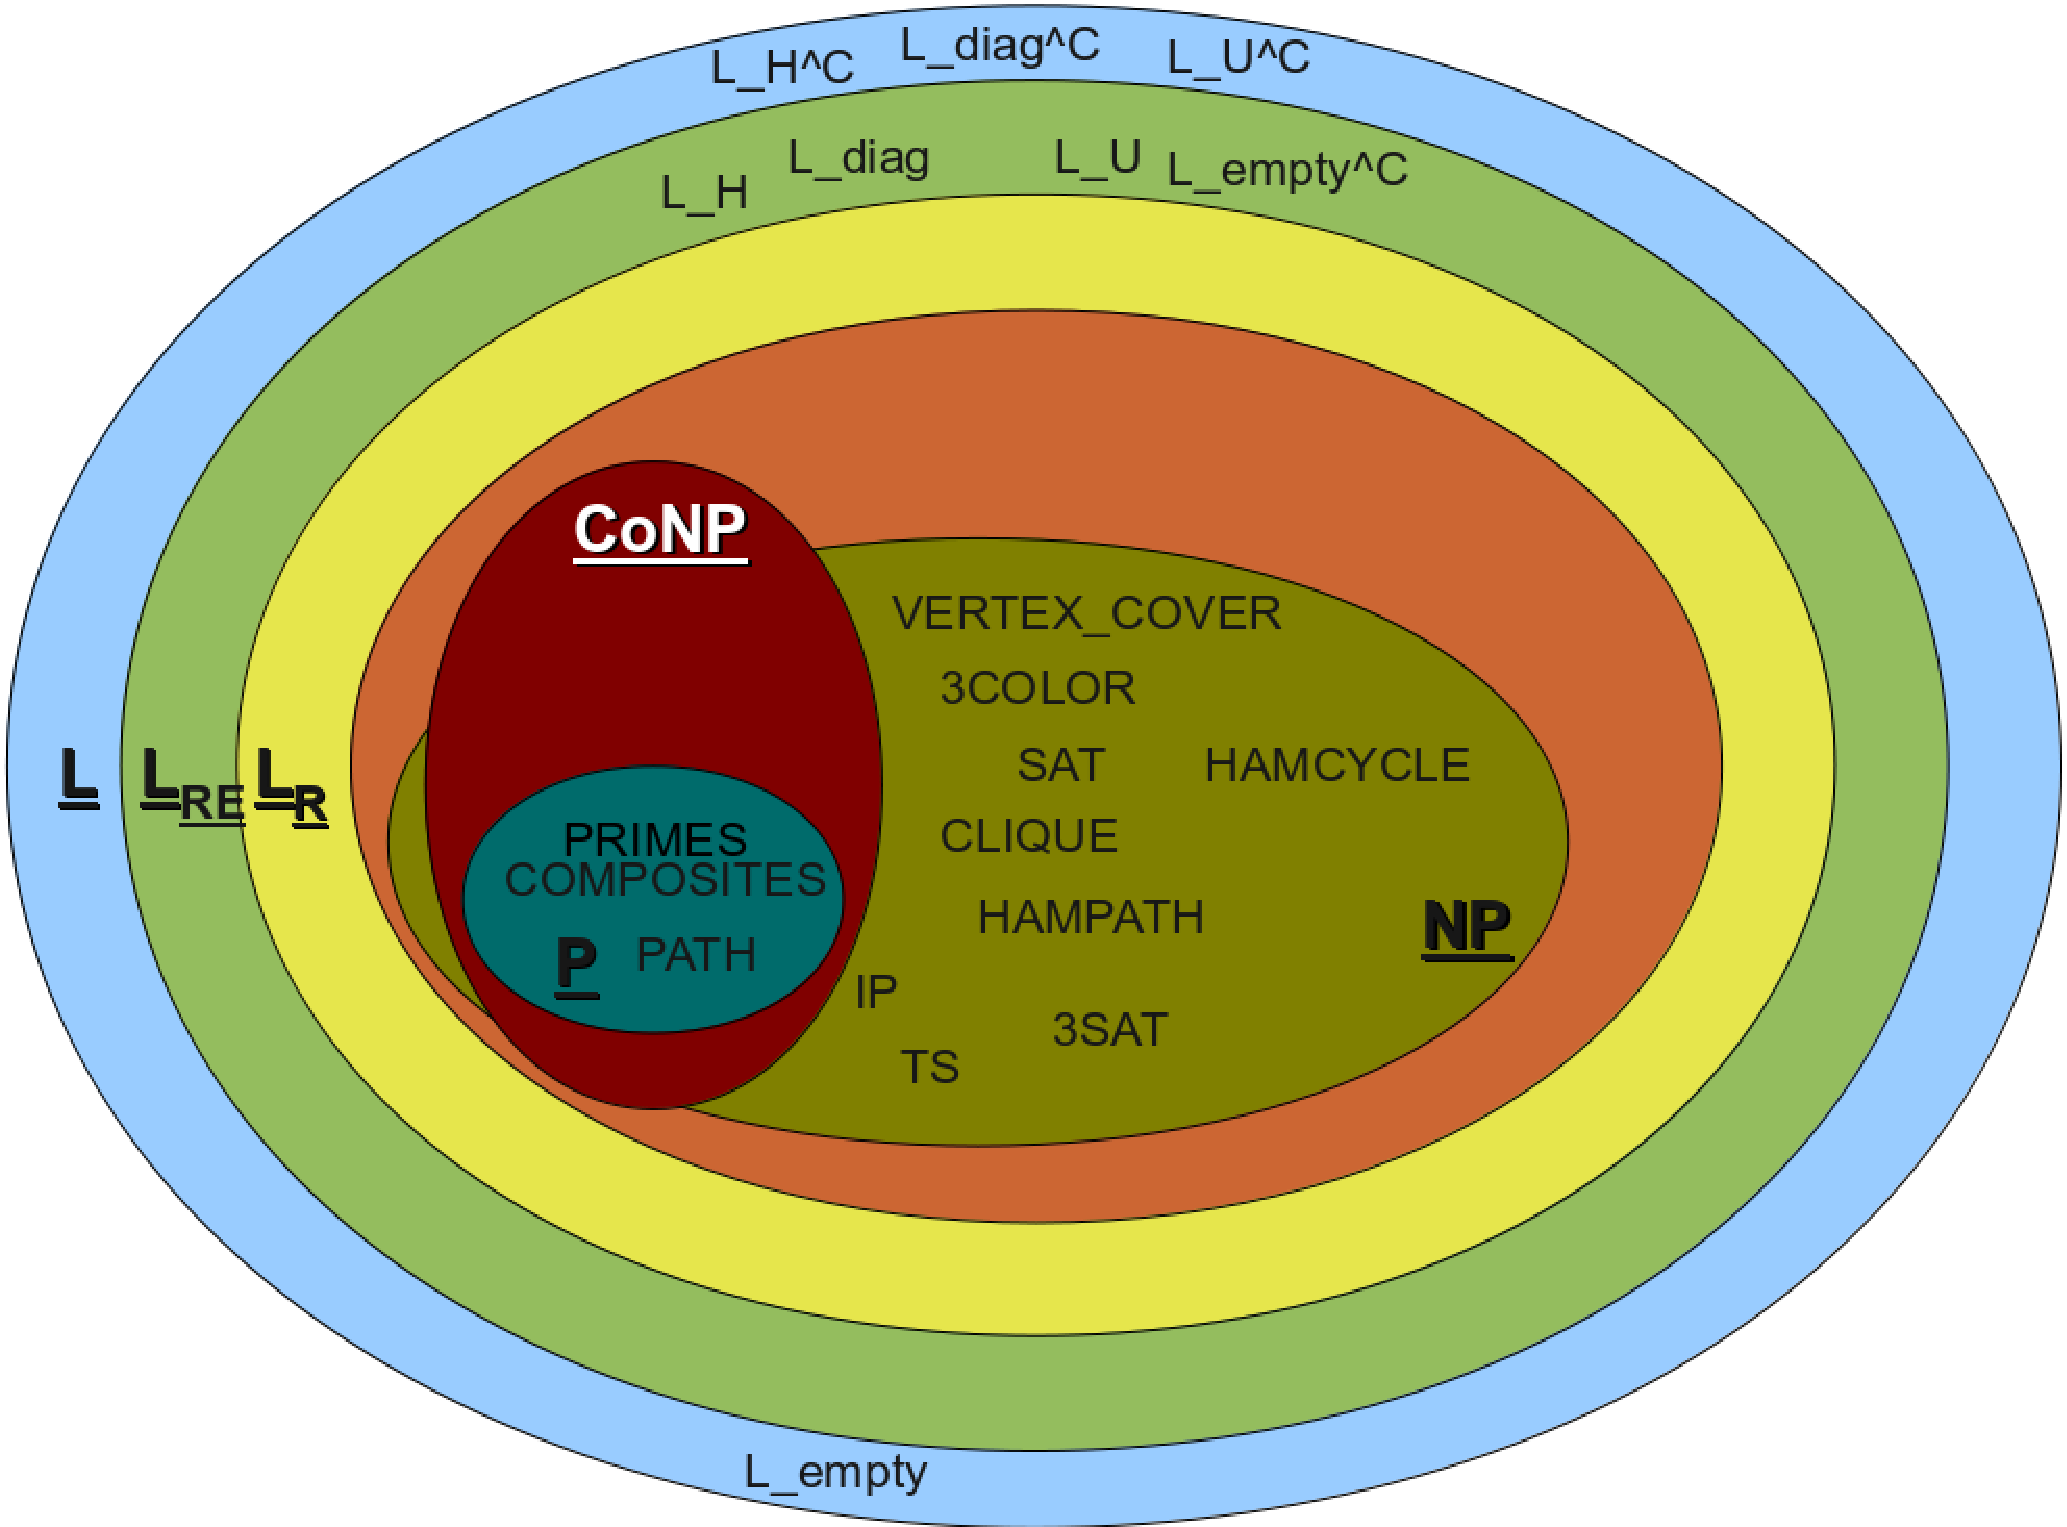
\includegraphics[scale=0.45]{cc.pdf}

\section*{Langages dans $\mathcal{L} \setminus \mathcal{L}_{RE}$}

\begin{itemize}
\item $L_{diag}^C = \left\{w \in \{0,1\}^* \mid w = w_i \text{ pour un certain }i \text{ et } M_i \text{ n'accepte pas } 
w_i\right\}$
\item $L_U^C = \left\{w \in \Sigma^*_{bool} \mid w = Kod(M)\#x \text{ pour une certaine machine M et un certain mot x tels 
que M refuse x}\right\} $
\item $L_H^C = \{w \in \Sigma^*_{bool} \mid w = Kod(M)\#x $ pour une certaine machine M et un certain mot x tels 
que M ne \indent$\qquad\,\,\, $ s'arrête pas sur x$\} $
\item $L_{empty} = \{ x \mid x = Kod(M)$ et $L(M)=\emptyset\}$
\end{itemize}

\section*{Langages dans $\mathcal{L}_{RE} \setminus \mathcal{L}_{R}$}

\begin{itemize}
\item $L_{diag} = \left\{w \in \{0,1\}^* \mid w = w_i \text{ pour un certain }i \text{ et } M_i \text{ accepte } w_i\right\}$
\item $L_U = \left\{w \in \Sigma^*_{bool} \mid w = Kod(M)\#x \text{ pour une certaine machine M et un certain mot x tels 
que M accepte x}\right\} $
\item $L_H = \{w \in \Sigma^*_{bool} \mid w = Kod(M)\#x $ pour une certaine machine M et un certain mot x tels 
que M \indent$\qquad\,\,\, $ s'arrête sur x$\} $
\item $L_{empty}^C = \{ x \mid x = Kod(M)$ et $L(M)\neq\emptyset\}$
\end{itemize}

\section*{Problèmes dans P}

\noindent $PATH = \{ <G,s,t> \mid G$ est un graphe orienté, $s$ et $t$ des sommets de $G$ tels que $\exists$ un chemin de $s$ à 
$t \}$ \\
$COMPOSITES = \{ <n> \mid n$ est un nombre composé $\}$ \\
$PRIMES = COMPOSITE^C = \{ <n> \mid n$ est un nombre premier $\}$ \\
\newpage

\section*{Problèmes dans NP \textit{(NP-complet)}}

\begin{itemize}
\item $HAMPATH = \{ <G,s,t> \mid G$ est un graphe orienté, $s$ et $t$ des sommets de $G$ tels que $\exists$ un chemin 
\indent$\qquad\,\,\,\,\,\qquad\qquad$ hamiltonien de $s$ à $t$ (en passant une et une seule fois par chaque chemin)$\}$
\item $CLIQUE = \{ <G,k> \mid G$ graphe non-orienté, $k$ un entier tel que $G$ contient une clique de taille $k\}$
\item $SAT = \{ <\varphi> \mid \varphi$ est une formule booléenne satisfaisable$\}$
\item $3SAT = \{ <\varphi> \mid \varphi$ est une formule booléenne satisfaisable écrite sous la forme d'une conjonction 
\indent$\qquad\,\,\,\,\,$ de clauses. Chaque clause étant une disjonction de 3 littéraux, un littéral étant soit une
variable \indent$\qquad\,\,\,\,\,$ booléenne ou sa négation.$\}$
\item $VERTEX\_COVER = \{ <G,k> \mid G$ graphe non-orienté possédant une couverture de taille $k \}$
\item $HAMCYCLE = \{ <G> \mid G$ graphe non-orienté possédant un cycle Hamiltonien$\}$
\item $TS = \{ <G,k> \mid G$ graphe non-orienté complet pondéré par des naturels tel que $G$ possède un cycle \indent$\qquad\,\,
\,$ hamiltonien de coût $\leq k\}$
\item $IP = \{ <A,\overrightarrow{b}> \mid A$ matrice $m\times n$ d'entiers, $\overrightarrow{b}$ vecteur de $m$ entiers tels 
que $\exists \overrightarrow{x}$ vecteur d'entiers satisfaisant $A\overrightarrow{x} \geq \overrightarrow{b}\}$
\item $3COLOR = \{ <G> | G$ est $3$-colorable $\}$
\end{itemize}

\end{sffamily}\end{document}